\documentclass[11pt,a4paper]{article}

% --- Codificacion e idioma ---
\usepackage[utf8]{inputenc}
\usepackage[T1]{fontenc}
\usepackage[spanish,es-tabla]{babel}

% --- Geometria y tipografia ---
\usepackage[margin=2.4cm, headheight=14pt]{geometry}
\usepackage{lmodern}
\usepackage{microtype}
\usepackage{parskip}
\setlength{\parindent}{0pt}

% --- Matematicas y tablas ---
\usepackage{amsmath, amssymb, amsthm}
\usepackage{booktabs}
\usepackage{array}
\usepackage{multirow}
\usepackage{siunitx}

% --- Graficos y cajas didacticas ---
\usepackage{graphicx}
\usepackage{float}
\usepackage{xcolor}
\usepackage{tcolorbox}
\tcbuselibrary{skins, breakable}
\usepackage{tikz}
\usetikzlibrary{arrows.meta, positioning, shapes.geometric, fit, calc}

% --- Enlaces y encabezados ---
\usepackage{fancyhdr}
\usepackage{enumitem}
\usepackage[colorlinks=true, linkcolor=azulInst, urlcolor=azulSec, citecolor=azulInst]{hyperref}

% --- Paleta de colores ---
\definecolor{azulInst}{HTML}{1B365D}
\definecolor{azulSec}{HTML}{2C5E8A}
\definecolor{grisFondo}{HTML}{F4F6F9}
\definecolor{verdeNota}{HTML}{1E6B52}
\definecolor{ambarAlerta}{HTML}{9A5B13}

% --- Encabezados y pies de pagina ---
\pagestyle{fancy}
\fancyhf{}
\fancyhead[L]{\small\color{azulInst}\textbf{Módulo 1:} Pronóstico de Demanda y Planeación de Flota}
\fancyhead[R]{\small\color{gray}Lectura Teórico--Metodológica}
\fancyfoot[C]{\small\thepage}
\renewcommand{\headrulewidth}{0.4pt}

% --- Cajas didacticas ---
\newtcolorbox{cajaConcepto}[1]{
    enhanced, breakable,
    colback=grisFondo, colframe=azulInst,
    fonttitle=\bfseries\color{white},
    colbacktitle=azulInst,
    title={#1},
    boxrule=0.8pt, arc=3pt, left=8pt, right=8pt, top=6pt, bottom=6pt
}

\newtcolorbox{cajaAlerta}[1]{
    enhanced, breakable,
    colback=ambarAlerta!5!white, colframe=ambarAlerta,
    colbacktitle=ambarAlerta,
    fonttitle=\bfseries\color{white},
    title={#1},
    boxrule=0.8pt, arc=3pt, left=8pt, right=8pt, top=6pt, bottom=6pt
}

\newtcolorbox{cajaIntuicion}[1]{
    enhanced, breakable,
    colback=verdeNota!5!white, colframe=verdeNota,
    colbacktitle=verdeNota,
    fonttitle=\bfseries\color{white},
    title={#1},
    boxrule=0.8pt, arc=3pt, left=8pt, right=8pt, top=6pt, bottom=6pt
}

\title{
    \vspace{-1cm}
    {\color{azulInst}\rule{\linewidth}{1.5pt}}\\[0.4cm]
    {\Huge\bfseries\color{azulInst} Estructuración del Modelo de Pronóstico de Demanda y Resultados de Referencia}\\[0.25cm]
    {\Large\color{azulSec} Módulo 1: Transporte Intermunicipal de Pasajeros por Carretera en Colombia}\\[0.2cm]
    {\color{azulInst}\rule{\linewidth}{0.8pt}}
}
\author{Material de Lectura Teórico--Explicativa $\cdot$ Redes Neuronales (Trabajo 3)}
\date{Basado en datos reales de \texttt{modulo1\_demanda} (2021--2026)}

\begin{document}

\maketitle
\thispagestyle{empty}

\begin{abstract}
\noindent El pronóstico de demanda diaria de pasajeros a un horizonte de 30 días sobre una red nacional de 848 rutas intermunicipales presenta desafíos estadísticos y operativos no triviales: conteos discretos no negativos con fuerte asimetría positiva, múltiples estacionalidades superpuestas (semanal, anual y calendario festivo colombiano), discontinuidades históricas en los registros (hueco estructural en 2024) y la necesidad de cuantificar incertidumbre mediante cuantiles para dimensionar flota y conductores. Esta lectura explica de forma progresiva y rigurosa: (1) la estructura física y temporal de los datos proporcionados, (2) la formulación causal sin fuga de información, (3) la fundamentación matemática de los modelos de referencia (Ingenuo Estacional, GLM Poisson Global y GLM Poisson Específico por Ruta), (4) la calibración conformalizada de cuantiles por nivel de volumen, (5) su acoplamiento con la planeación operativa de flota, y (6) la interpretación de los resultados empíricos obtenidos como línea base para modelos de redes neuronales.
\end{abstract}

\tableofcontents
\newpage

% ==============================================================================
\section{Introducción y Planteamiento del Problema}
% ==============================================================================

En la operación de transporte intermunicipal de pasajeros por carretera, la toma de decisiones diaria (cuántos vehículos despachar, de qué tipología y cuántos conductores programar) depende de anticipar la demanda futura con suficiente antelación. Un horizonte operativo estándar de planeación es $H = 30$ días calendario: permite coordinar turnos semanales de conductores, mantenimientos preventivos de flota y refuerzos en temporadas altas.

Sin embargo, modelar esta demanda no es un ejercicio estándar de regresión lineal por cuatro razones fundamentales:
\begin{enumerate}[leftmargin=1.5em]
    \item \textbf{Naturaleza de conteo y heterocedasticidad:} la variable objetivo $Y_{r,t}$ representa pasajeros diarios en una ruta dirigida $r$ en la fecha $t$. Es un entero no negativo ($Y_{r,t} \in \mathbb{Z}_{\ge 0}$) cuya varianza crece con la media y cuya distribución presenta colas derechas pronunciadas en puentes festivos y vacaciones.
    \item \textbf{Heterogeneidad espacial y direccional:} la red analizada consta de $R = 848$ rutas dirigidas con escalas radicalmente distintas (desde rutas regionales de $\approx 25$ pasajeros/día hasta corredores metropolitanos como \textit{Medellín $\to$ Rionegro} con $2{,}947.7$ pax/día en promedio). Además, una ruta de \textit{Ida} (ej. \textit{Bogotá $\to$ Villavicencio}) tiene una dinámica de calendario opuesta a su \textit{Regreso} (\textit{Villavicencio $\to$ Bogotá}) al inicio y final de un puente festivo.
    \item \textbf{Riesgo de fuga de información (\textit{data leakage}):} si se entrena un modelo para predecir el día $t_0 + 25$ usando el rezago de hace 7 días ($Y_{r, t_0+18}$), el modelo parecerá muy preciso en validación histórica pero será inútil en producción, pues en el origen $t_0$ el día $t_0+18$ aún pertenece al futuro.
    \item \textbf{Decisiones bajo incertidumbre asimétrica:} planear la flota con el valor esperado (media o mediana $P_{50}$) implica quedarse corto en el $50\%$ de los días, dejando pasajeros en terminal. Por ello, la salida requerida no es solo un punto, sino una distribución predictiva expresada en cuantiles ($P_{05}, P_{10}, P_{50}, P_{75}, P_{90}, P_{95}$).
\end{enumerate}

% ==============================================================================
\section{Naturaleza de los Datos y Construcción de Series Temporales}
% ==============================================================================

\subsection{Fuentes primarias y definición de ruta}

Los datos provienen de dos fuentes oficiales en Colombia:
\begin{itemize}[leftmargin=1.5em]
    \item \textbf{Superintendencia de Transporte} (\texttt{datos.gov.co}, conjunto \texttt{eh75-8ah6}): registros de despacho de vehículos y pasajeros movilizados por terminal terrestre.
    \item \textbf{DANE -- DIVIPOLA} (\texttt{datos.gov.co}, conjunto \texttt{gdxc-w37w}): codificación oficial de municipios (5 dígitos) y sus coordenadas geográficas $(\text{lat}, \text{lon})$.
\end{itemize}

Cada ruta dirigida se identifica mediante la llave \texttt{ruta\_id} $= \text{DIVIPOLA}_{\text{origen}}\_\text{DIVIPOLA}_{\text{destino}}$. Por ejemplo, \texttt{11001\_50001} corresponde a \textit{Bogotá, D.C. $\to$ Villavicencio}, mientras que \texttt{50001\_11001} representa el sentido inverso (\textit{Villavicencio $\to$ Bogotá, D.C.}). A partir de las coordenadas DIVIPOLA se calcula la distancia geodésica en línea recta $d_r$ (fórmula de Haversine), que varía desde trayectos cortos de cercanía hasta corredores troncales de cientos de kilómetros.

\subsection{Despachos en \texttt{ORIGEN} vs. \texttt{TRANSITO}}

Un aspecto crítico en el diseño de los datos (\texttt{src/build\_dataset.py}) es la separación estricta entre dos tipos de registro en terminal:
\begin{itemize}[leftmargin=1.5em]
    \item \textbf{\texttt{ORIGEN}:} pasajeros que abordan el vehículo al inicio del viaje en esa terminal. Constituye la \textbf{variable objetivo} ($Y_{r,t} = \texttt{pasajeros\_origen}$), pues representa la demanda primaria generada en el municipio de origen que requiere capacidad de despacho propia.
    \item \textbf{\texttt{TRANSITO}:} pasajeros que pasan por la terminal en rutas de paso procedentes de otro origen. Sumar ambos provocaría doble conteo en la red. Por ello, \texttt{pasajeros\_transito} se mantiene separado y solo ingresa como \textbf{señal exógena rezagada} (promedio móvil de 28 días rezagado 30 días), capturando la presión de ocupación previa en corredores compartidos (ej. \textit{Bogotá $\to$ Cali} con $1{,}217.8$ pax/día en origen y $2{,}299.2$ pax/día en tránsito).
\end{itemize}

\subsection{Selección de rutas activas y estructura en bloques continuos}

Para garantizar series estadísticamente modelables y evitar ruido de rutas esporádicas o errores de digitación geográfica, se aplican cuatro filtros reproducibles:
\begin{enumerate}[leftmargin=1.5em]
    \item Al menos $500$ días con registro \texttt{ORIGEN} en el bloque histórico $2021\text{--}2023$.
    \item Promedio diario $\ge 25$ pasajeros en el bloque $2021\text{--}2023$.
    \item Al menos $60$ días con registro \texttt{ORIGEN} en el bloque reciente $2026$ (enero--marzo).
    \item Exclusión de anomalías DIVIPOLA documentadas (como \texttt{76001\_47570}, Cali $\to$ Puebloviejo a $878\text{ km}$ reportada en buseta) o municipios sin coordenadas válidas.
\end{enumerate}

Tras estos filtros se consolidan exactamente \textbf{$R = 848$ rutas dirigidas}. El panel resultante (\texttt{series\_diarias.parquet}) contiene \textbf{$1{,}286{,}416$ filas} organizadas en \textbf{tres bloques temporales continuos} (\texttt{bloque\_id}), excluyendo explícitamente el hueco estructural de 2024 y el corte parcial de diciembre de 2025:

\begin{table}[H]
\centering
\caption{Estructura de bloques continuos en \texttt{series\_diarias.parquet} ($R=848$ rutas).}
\label{tab:bloques}
\begin{tabular}{llrrrrr}
\toprule
\textbf{Bloque} & \textbf{Rango de fechas} & \textbf{Filas totales} & \textbf{Con registro} & \textbf{Media pax/día} & \textbf{Mediana pax/día} \\
\midrule
\texttt{B1\_2021\_2023} & 2021-01-01 a 2023-12-31 & $928{,}560$ & $895{,}574$ & $231.67$ & $98.0$ \\
\texttt{B2\_2025}      & 2025-01-01 a 2025-11-29 & $282{,}384$ & $279{,}441$ & $278.17$ & $119.0$ \\
\texttt{B3\_2026}      & 2026-01-01 a 2026-03-30 & $75{,}472$  & $72{,}501$  & $262.82$ & $110.0$ \\
\midrule
\textbf{Total}         &                         & \textbf{1,286,416} & \textbf{1,247,516} & --- & --- \\
\bottomrule
\end{tabular}
\end{table}

\begin{cajaAlerta}{¿Por qué respetar los límites de cada \texttt{bloque\_id} al calcular rezagos?}
Si se concatenaran \texttt{B1\_2021\_2023} y \texttt{B2\_2025} como si fueran días consecutivos, el cálculo de un rezago de 35 días en enero de 2025 leería erróneamente datos de noviembre de 2023. Por esta razón, todos los operadores de rezago (\texttt{shift}) y ventanas móviles (\texttt{rolling}) se calculan particionados por $(\texttt{ruta\_id}, \texttt{bloque\_id})$. Adicionalmente, la marca \texttt{dia\_sin\_registro\_origen} distingue los días sin reporte en terminal para excluirlos del ajuste de parámetros y evitar sesgar la demanda hacia cero.
\end{cajaAlerta}

Observemos la diferencia entre la media ($231\text{--}278$ pax/día) y la mediana ($98\text{--}119$ pax/día) en la Tabla~\ref{tab:bloques}: la media duplica con creces a la mediana, lo que confirma una \textbf{fuerte asimetría positiva} en la distribución de la demanda. La Figura~\ref{fig:eda_cobertura} ilustra la cobertura mensual histórica y el hueco estructural de 2024, mientras que la Figura~\ref{fig:eda_stl} muestra la descomposición estacional (tendencia, componente semanal/anual y residuos) en el corredor troncal \textit{Bogotá $\to$ Cali}.

\begin{figure}[H]
\centering
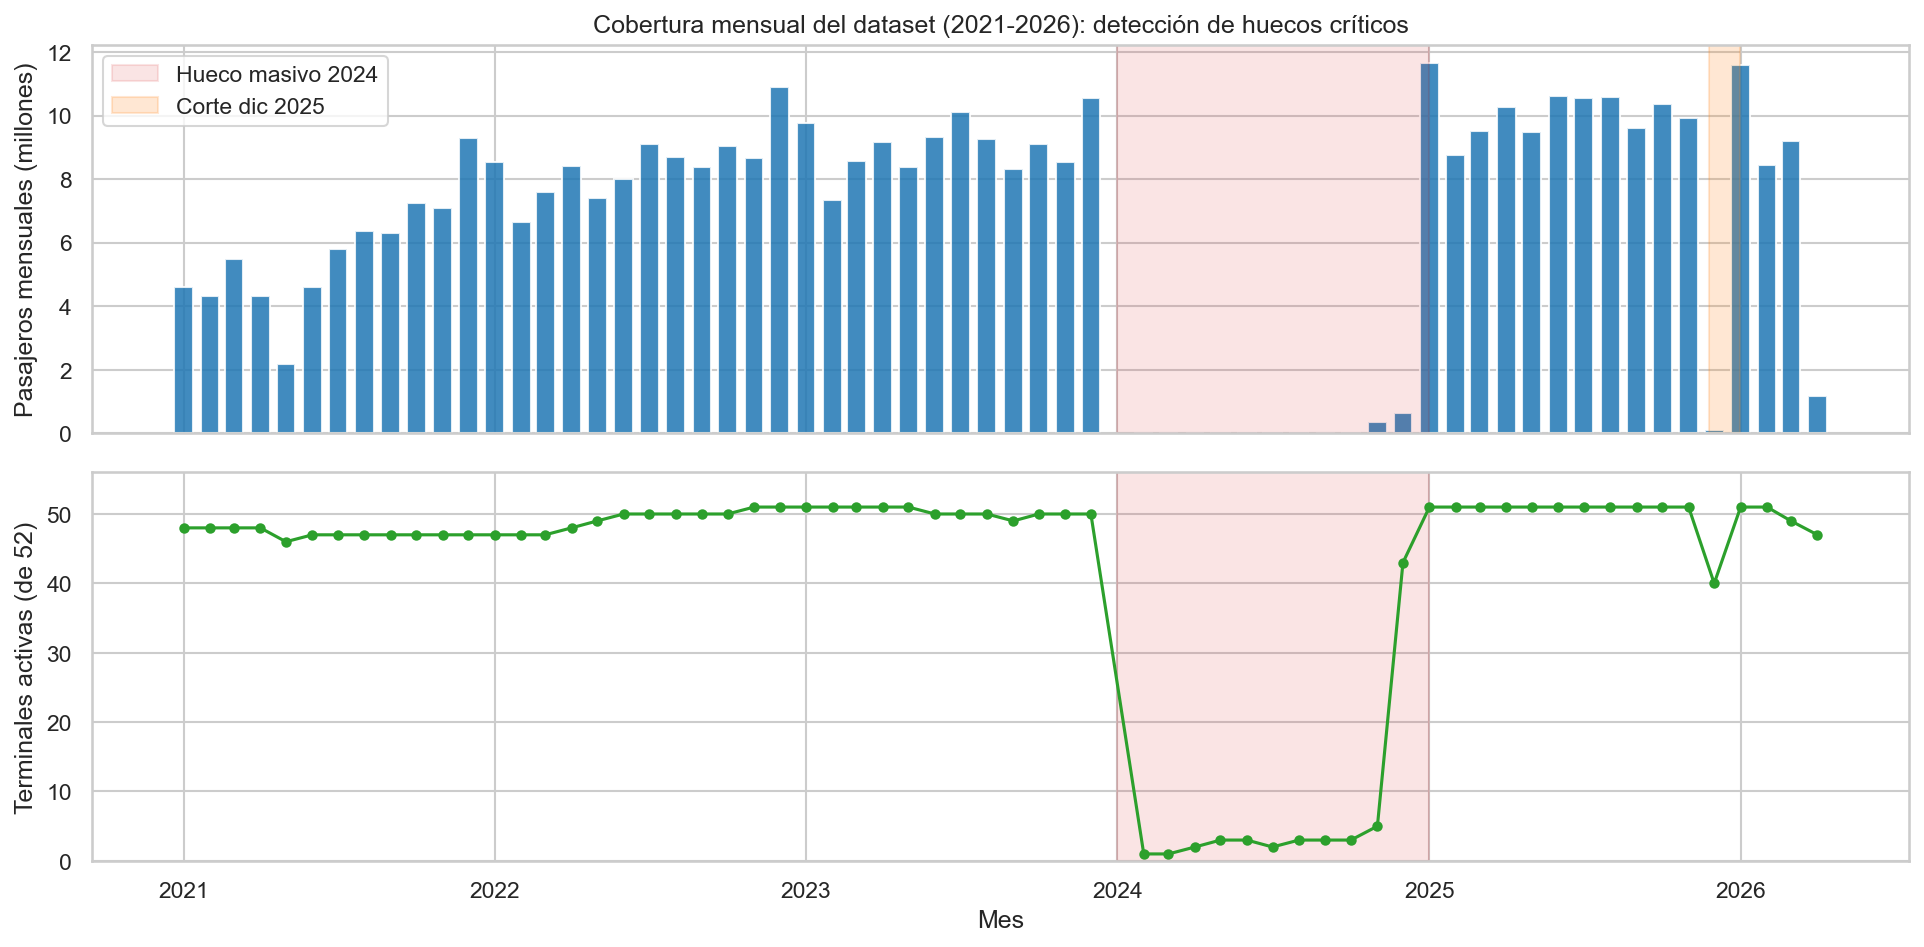
\includegraphics[width=0.92\linewidth]{../figures/eda_01_cobertura_mensual.png}
\caption{Cobertura mensual de registros operativos en la serie histórica, evidenciando los bloques continuos válidos y el vacío estructural de 2024.}
\label{fig:eda_cobertura}
\end{figure}

\begin{figure}[H]
\centering
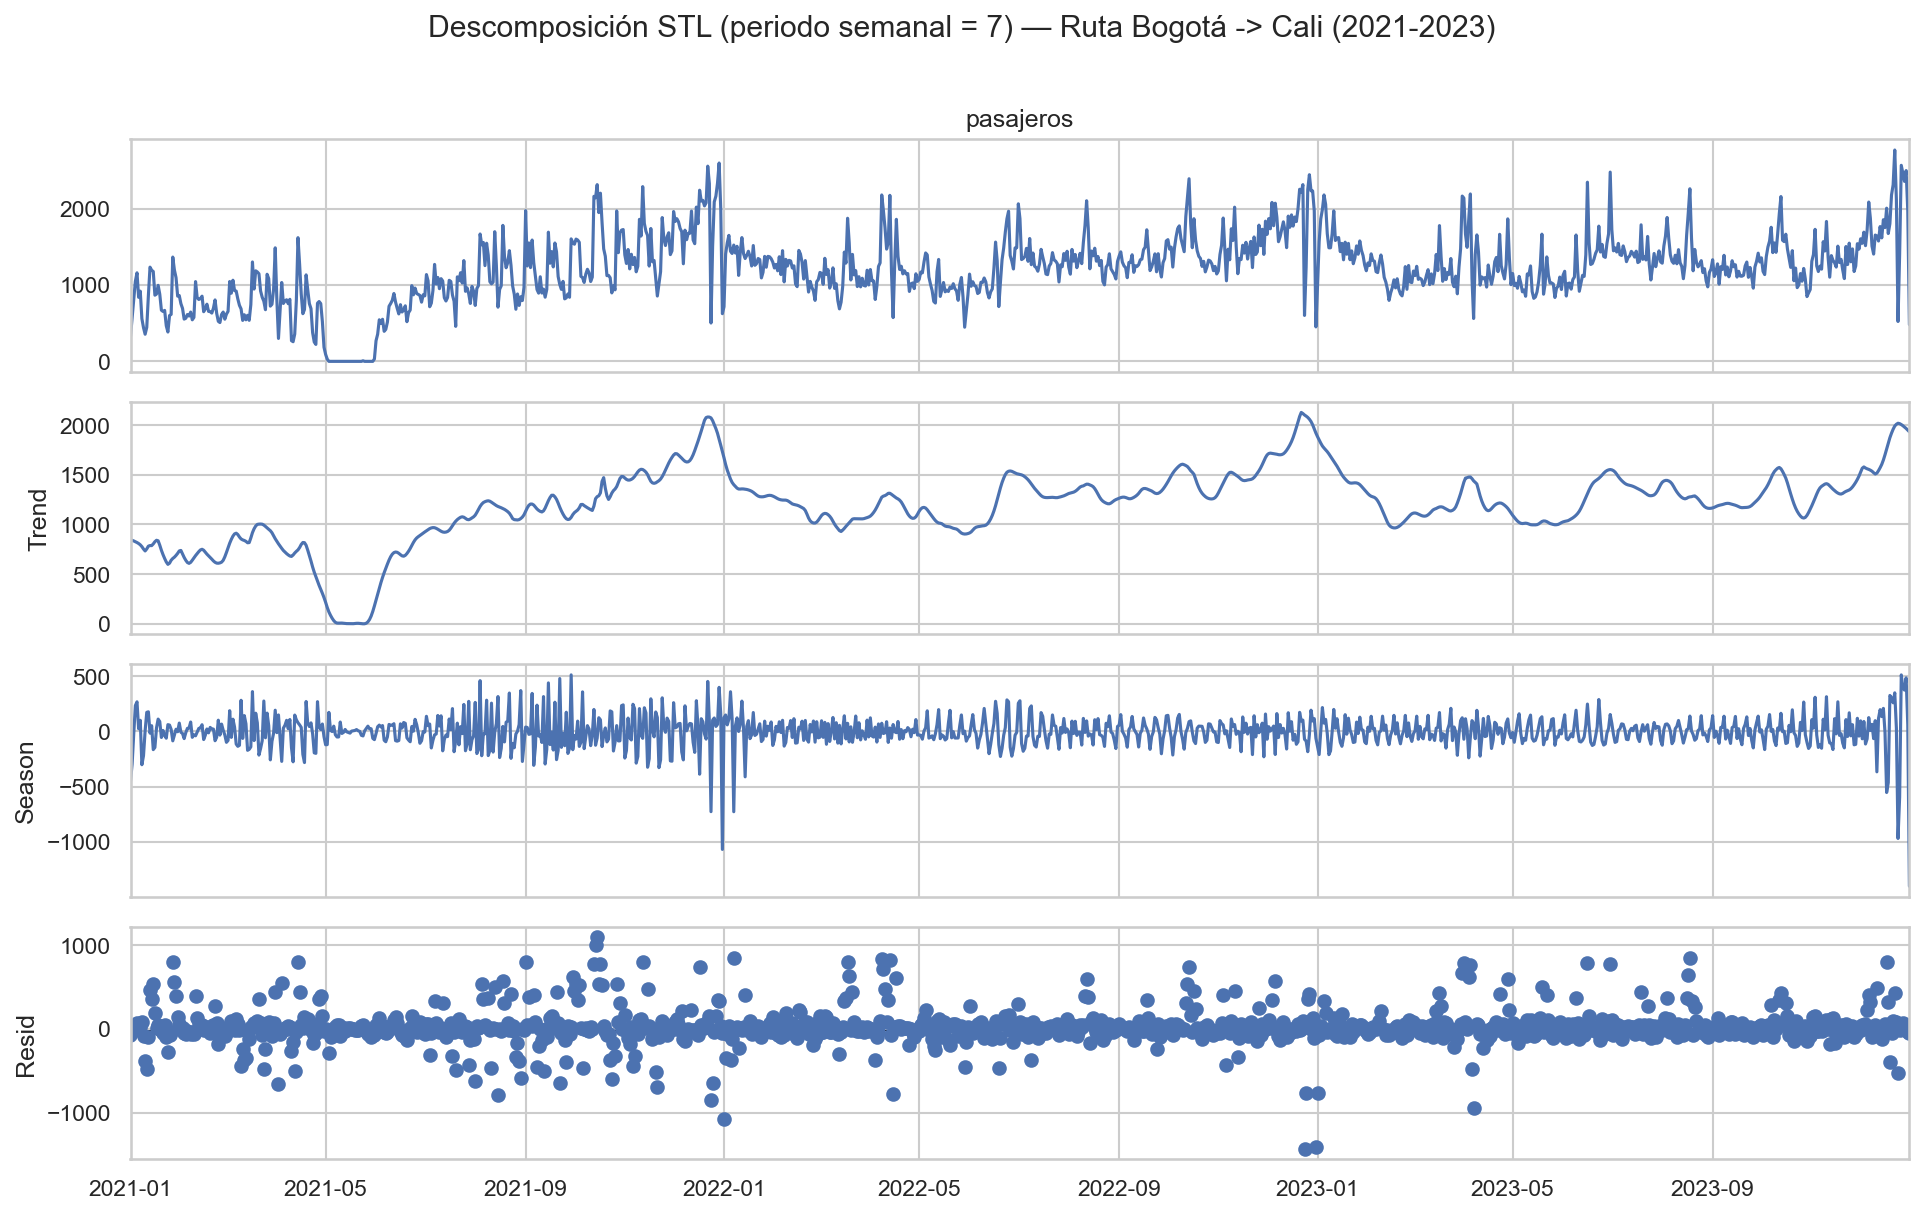
\includegraphics[width=0.92\linewidth]{../figures/eda_08_descomposicion_stl_bog_cali.png}
\caption{Descomposición STL de la demanda diaria en la ruta \textit{Bogotá, D.C. $\to$ Santiago de Cali}, mostrando tendencia de largo plazo, estacionalidad semanal y picos de calendario.}
\label{fig:eda_stl}
\end{figure}

\subsection{Ingeniería de calendario colombiano}

En Colombia, la demanda de transporte intermunicipal está gobernada por un calendario festivo particular, implementado de forma determinista en \texttt{src/calendario.py}:
\begin{itemize}[leftmargin=1.5em]
    \item \textbf{Ley 51 de 1983 (Ley Emiliani):} establece 18 festivos nacionales al año (fijos, religiosos móviles dependientes del Domingo de Pascua mediante el algoritmo de Meeus/Jones/Butcher, y festivos trasladados al lunes siguiente).
    \item \textbf{Efecto puente completo (\texttt{es\_puente}):} marca no solo el lunes festivo, sino también el viernes de salida, sábado y domingo asociados, pues la movilidad se redistribuye en los cuatro días.
    \item \textbf{Vísperas y temporadas especiales:} \texttt{es\_vispera\_festivo} (día previo a festivo), \texttt{es\_semana\_santa} (Domingo de Ramos a Domingo de Pascua), \texttt{es\_receso\_octubre} (Decreto 1373 de 2007: semana anterior al festivo del Día de la Raza), \texttt{es\_temporada\_fin\_anio} (15 de diciembre a 12 de enero) y \texttt{es\_temporada\_mitad\_anio} (15 de junio a 15 de julio).
\end{itemize}
Todas estas variables son \textbf{exógenas deterministas} conocidas con años de anticipación, por lo que pueden evaluarse en cualquier horizonte futuro $t_0 + h$ sin riesgo de fuga de información.

% ==============================================================================
\section{Formulación Causal y Prevención de Fuga de Información}
% ==============================================================================

Sea $t_0$ el origen del pronóstico (último día observado antes de la ventana de predicción) y $h \in \{1, 2, \dots, 30\}$ el horizonte en días. El objetivo es estimar la distribución condicional de $Y_{r, t_0+h}$ dada la información disponible hasta $t_0$:
\[
\mathcal{F}_{r, t_0} = \big\{ Y_{r, s},\, Y^{\text{tránsito}}_{r, s} : s \le t_0 \big\} \;\cup\; \big\{ \mathbf{c}_{t_0+h},\, d_r \big\},
\]
donde $\mathbf{c}_{t_0+h}$ representa las variables deterministas de calendario en la fecha objetivo y $d_r$ la distancia de la ruta.

\begin{cajaConcepto}{Regla estricta de causalidad para horizonte $H=30$ días}
Si un modelo tabulado utiliza una sola estructura de características para predecir simultáneamente los días $h = 1, 2, \dots, 30$ de una ventana de prueba, \textbf{todo rezago de la variable objetivo debe ser de al menos $30$ días} ($k \ge 30$). De lo contrario, al evaluar $h = 20$, un rezago de $7$ días estaría leyendo el valor real de $t_0 + 13$, cometiendo fuga de información.
\end{cajaConcepto}

En \texttt{src/modelos\_referencia.py}, la función \texttt{preparar\_features\_sin\_fuga} garantiza esta propiedad construyendo únicamente rezagos semanales múltiplos de 7 con $k \ge 35$ y estadísticas móviles desplazadas 30 días hacia el pasado:

\begin{itemize}[leftmargin=1.5em]
    \item \textbf{Rezagos semanales profundos:} $\text{lag}_{35}, \text{lag}_{42}, \text{lag}_{49}, \text{lag}_{56}$ transformados con $\log(1+x)$. Preservar múltiplos de 7 asegura que al predecir un viernes, los rezagos correspondan también a viernes anteriores (5, 6, 7 y 8 semanas atrás).
    \item \textbf{Tendencia y volatilidad reciente sin fuga:} promedio móvil de 7 días (\texttt{roll7\_lag30}), promedio móvil de 28 días (\texttt{roll28\_lag30}), desviación estándar de 28 días (\texttt{std28\_lag30}) y tránsito promedio de 28 días (\texttt{transito\_roll28\_lag30}), todos desplazados mediante \texttt{shift(30)} y transformados con $\log(1+x)$.
    \item \textbf{Codificación cíclica de Fourier:} para evitar discontinuidades artificiales entre domingo ($6$) y lunes ($0$) o entre el 31 de diciembre ($365$) y el 1 de enero ($1$), se proyecta el ciclo semanal y anual sobre el círculo unitario:
    \[
    \sin\!\left(\frac{2\pi \cdot \text{día\_sem}}{7}\right),\; \cos\!\left(\frac{2\pi \cdot \text{día\_sem}}{7}\right),\qquad
    \sin\!\left(\frac{2\pi \cdot \text{día\_año}}{365.25}\right),\; \cos\!\left(\frac{2\pi \cdot \text{día\_año}}{365.25}\right).
    \]
    \item \textbf{Variables categóricas e indicadores de calendario:} codificación \textit{one-hot} de \texttt{dia\_semana\_num} y \texttt{mes} (más \texttt{ruta\_id} en el modelo global), junto con las 8 banderas binarias de calendario y $\log(1 + d_r)$ en el modelo global.
\end{itemize}

\subsection{Partición temporal de entrenamiento, validación y prueba}

Para evaluar la capacidad de generalización en condiciones reales y en distintos regímenes de calendario, el dataset se divide cronológicamente (sin mezcla aleatoria):
\begin{itemize}[leftmargin=1.5em]
    \item \textbf{Entrenamiento (\texttt{train}):} desde el inicio válido (tras los primeros 56 días de calentamiento de rezagos) hasta \texttt{2023-12-31}, más \texttt{2025-01-01} a \texttt{2025-07-31}.
    \item \textbf{Validación (\texttt{val}):} \texttt{2025-08-01} a \texttt{2025-09-30} (2 meses usados para seleccionar el modelo ganador y calibrar los cuantiles conformalizados).
    \item \textbf{Prueba (\texttt{test}):} tres ventanas disjuntas de 30 días ($h = 1 \dots 30$):
    \begin{enumerate}
        \item \texttt{W1\_Oct2025\_Receso} (\texttt{2025-10-01} a \texttt{2025-10-30}): evalúa el receso escolar de octubre.
        \item \texttt{W2\_Nov2025\_Puentes} (\texttt{2025-10-31} a \texttt{2025-11-29}): evalúa la secuencia de puentes festivos de noviembre.
        \item \texttt{W3\_Mar2026\_Reciente} (\texttt{2026-03-01} a \texttt{2026-03-30}): evalúa el desempeño más reciente (incluyendo Semana Santa 2026 al cierre de marzo) y genera el archivo operativo \texttt{pronosticos\_30d.csv}.
    \end{enumerate}
\end{itemize}

% ==============================================================================
\section{Estructuración Teórica de los Modelos de Referencia}
% ==============================================================================

Antes de entrenar arquitecturas neuronales complejas, es indispensable construir modelos de referencia (\textit{baselines}) sólidos, interpretables y libres de fuga. Se comparan tres enfoques en orden creciente de complejidad.

\subsection{Modelo 1: Ingenuo Estacional sin fuga (\textit{Seasonal Naive})}

Este modelo no estima parámetros; simplemente proyecta el último valor observado del mismo día de la semana que sea causalmente conocido en el origen $t_0$:
\[
\hat{Y}^{\text{ingenuo}}_{r, t_0+h} =
\begin{cases}
Y_{r, t_0 + h - 7}  & \text{si } 1 \le h \le 7, \\
Y_{r, t_0 + h - 14} & \text{si } 8 \le h \le 14, \\
Y_{r, t_0 + h - 21} & \text{si } 15 \le h \le 21, \\
Y_{r, t_0 + h - 28} & \text{si } 22 \le h \le 28, \\
Y_{r, t_0 + h - 35} & \text{si } 29 \le h \le 30.
\end{cases}
\]
Su virtud es capturar de forma inmediata la escala de cada ruta y su patrón semanal (ej. domingo vs. martes). Su defecto es ser ciego a los festivos móviles, puentes y tendencias recientes.

\subsection{¿Por qué Regresión Poisson (GLM) en lugar de Mínimos Cuadrados Ordinarios?}

Una regresión lineal clásica (MCO) asume $\mathbb{E}[Y|\mathbf{x}] = \mathbf{x}^\top \boldsymbol{\beta}$ con errores gaussianos homocedásticos. En demanda de pasajeros esto falla por tres motivos:
\begin{enumerate}[leftmargin=1.5em]
    \item Puede predecir valores negativos ($\hat{Y} < 0$) en días valle o rutas pequeñas.
    \item Asume efectos \textbf{aditivos}: si un puente suma $+150$ pasajeros en promedio global, sobreestimará brutalmente una ruta de 30 pax/día y subestimará una ruta de 2,500 pax/día.
    \item Ignora que la dispersión del error crece proporcionalmente con el volumen esperado.
\end{enumerate}

El \textbf{Modelo Lineal Generalizado (GLM) de Poisson} con función de enlace logarítmica resuelve los tres problemas de forma elegante:
\[
Y_{r,t} \mid \mathbf{x}_{r,t} \sim \text{Poisson}(\mu_{r,t}), \qquad \log(\mu_{r,t}) = \eta_{r,t} = \beta_0 + \mathbf{x}_{r,t}^\top \boldsymbol{\beta} \implies \mu_{r,t} = \exp(\beta_0 + \mathbf{x}_{r,t}^\top \boldsymbol{\beta}) > 0.
\]

\begin{cajaIntuicion}{Interpretación multiplicativa del enlace logarítmico}
En un GLM Poisson, los coeficientes operan de forma \textbf{multiplicativa} sobre la demanda esperada:
\[
\mu_{r,t} = \exp(\beta_0) \cdot \prod_{j=1}^{p} \exp(\beta_j x_{r,t,j}).
\]
Así, si el coeficiente de \texttt{es\_puente} es $\beta_{\text{puente}} = 0.315$, significa que un puente festivo multiplica la demanda esperada de la ruta por $\exp(0.315) \approx 1.37$ ($+37\%$), independientemente de si la ruta mueve 40 o 2,000 pasajeros diarios. Además, dado que las variables de rezago entran como $\log(1 + Y_{\text{lag}})$, un coeficiente $\beta_{\text{lag}}$ actúa como una \textbf{elasticidad} ($Y_{\text{lag}}^{\beta_{\text{lag}}}$).
\end{cajaIntuicion}

La estimación de $\boldsymbol{\beta}$ minimiza la \textbf{devianza de Poisson} regularizada con penalización $L_2$ (\textit{Ridge}) para evitar sobreajuste y estabilizar la convergencia numérica:
\[
\mathcal{L}(\boldsymbol{\beta}) = \sum_{i=1}^{N} \Big( \exp(\mathbf{x}_i^\top \boldsymbol{\beta}) - y_i (\mathbf{x}_i^\top \boldsymbol{\beta}) \Big) + \frac{\alpha}{2} \|\boldsymbol{\beta}\|_2^2.
\]

\subsection{Modelo 2 vs. Modelo 3: GLM Global frente a GLM Específico por Ruta}

La arquitectura del sistema enfrenta una disyuntiva clásica de modelado jerárquico (compromiso sesgo--varianza):

\begin{itemize}[leftmargin=1.5em]
    \item \textbf{GLM Poisson General (Global):} ajusta \textit{un único modelo} sobre todo el panel ($\sim 1$ millón de filas en entrenamiento, $\alpha = 10^{-3}$). Cada ruta recibe su propio intercepto mediante \textit{one-hot encoding} de \texttt{ruta\_id}, pero todas las 848 rutas \textbf{comparten los mismos coeficientes} $\boldsymbol{\beta}$ de día de la semana, mes, festivos y rezagos.
    \begin{itemize}
        \item \textit{Ventaja:} baja varianza de estimación al aprovechar toda la muestra nacional.
        \item \textit{Limitación (alto sesgo):} obliga a que rutas turísticas, laborales, de ida y de regreso reaccionen exactamente igual ante un festivo o un viernes.
    \end{itemize}
    \item \textbf{GLM Poisson Específico (Por Ruta):} ajusta \textit{848 modelos independientes}, uno por cada \texttt{ruta\_id}, con mayor regularización ($\alpha = 0.2$) para compensar que cada modelo dispone de $\sim 900\text{--}1{,}200$ días de entrenamiento.
    \begin{itemize}
        \item \textit{Ventaja:} captura la \textbf{asimetría direccional} real de la red. Como muestran los resultados de significancia de calendario (\texttt{significancia\_calendario.csv}), en \textit{Bogotá $\to$ Villavicencio} un festivo reduce la salida en $-28.5\%$ ($p < 10^{-4}$) mientras que un puente completo la dispara en $+37.0\%$; en cambio, en el sentido inverso (\textit{Villavicencio $\to$ Bogotá}), el día festivo mismo crece $+10.8\%$ por el retorno de viajeros.
        \item \textit{Desventaja:} no comparte información entre rutas similares si alguna sufre un cambio de régimen reciente.
    \end{itemize}
\end{itemize}

% ==============================================================================
\section{Cuantificación de Incertidumbre: Cuantiles Conformalizados}
% ==============================================================================

Un GLM Poisson estándar asume que $\text{Var}(Y) = \mu$, lo cual en la práctica subestima severamente la dispersión real de los datos de transporte (\textbf{sobredispersión}: $\text{Var}(Y) \gg \mu$, causada por eventos climáticos, cierres viales o variabilidad no observada). Usar intervalos teóricos de Poisson produciría bandas demasiado estrechas y baja cobertura real.

Para resolverlo sin supuestos paramétricos rígidos sobre la varianza, se implementa \textbf{calibración conformalizada de cuantiles en escala logarítmica} sobre el conjunto de validación (\texttt{val}), segmentada por \textbf{terciles de volumen} de la ruta:

\begin{enumerate}[leftmargin=1.5em]
    \item \textbf{Segmentación por nivel de volumen (\textit{tiers}):} usando la demanda media histórica de cada ruta en entrenamiento, se definen los terciles $Q_{1/3} = 71.29$ y $Q_{2/3} = 195.88$ pax/día:
    \[
    \text{tier}(r) =
    \begin{cases}
    \text{baja}  & \text{si } \bar{Y}_r \le 71.29, \\
    \text{media} & \text{si } 71.29 < \bar{Y}_r \le 195.88, \\
    \text{alta}  & \text{si } \bar{Y}_r > 195.88.
    \end{cases}
    \]
    \item \textbf{Residuos logarítmicos en validación:} para cada observación de validación en el segmento, se mide el error multiplicativo relativo en escala $\log(1+y)$:
    \[
    e_i = \log(1 + y_i) - \log(1 + \hat{\mu}_i).
    \]
    \item \textbf{Cálculo de \textit{offsets} empíricos:} para cada cuantil objetivo $q \in \{0.05, 0.10, 0.50, 0.75, 0.90, 0.95\}$, se extrae el cuantil empírico de los residuos de validación dentro de cada \textit{tier}:
    \[
    \delta_{q, \text{tier}} = \text{Quantile}_q\!\left(\{ e_i : i \in \text{Val} \cap \text{tier} \}\right).
    \]
    \item \textbf{Proyección en prueba:} cada predicción puntual $\hat{\mu}_{r,t}$ se transforma en el cuantil calibrado mediante:
    \[
    \hat{Y}^{(q)}_{r,t} = \max\!\Big(0,\; \exp\!\big(\text{clip}(\log(1+\hat{\mu}_{r,t}) + \delta_{q,\text{tier}(r)},\; 0,\; 12)\big) - 1\Big).
    \]
\end{enumerate}

\begin{table}[H]
\centering
\caption{Offsets conformalizados ($\delta_{q, \text{tier}}$) calibrados en validación para el modelo ganador (\texttt{GLM\_Poisson\_Especifico\_PorRuta}).}
\label{tab:offsets}
\begin{tabular}{lrrrrrr}
\toprule
\textbf{Nivel de volumen (\textit{Tier})} & $P_{05}$ & $P_{10}$ & $P_{50}$ & $P_{75}$ & $P_{90}$ & $P_{95}$ \\
\midrule
\textbf{Baja} ($\le 71.3$ pax/día)    & $-0.9334$ & $-0.6465$ & $-0.0023$ & $+0.2253$ & $+0.4473$ & $+0.6068$ \\
\textbf{Media} ($71.3\text{--}195.9$) & $-0.7625$ & $-0.4466$ & $+0.0023$ & $+0.1690$ & $+0.3426$ & $+0.4717$ \\
\textbf{Alta} ($> 195.9$ pax/día)     & $-0.4528$ & $-0.3088$ & $-0.0091$ & $+0.1198$ & $+0.2624$ & $+0.3677$ \\
\bottomrule
\end{tabular}
\end{table}

La Tabla~\ref{tab:offsets} revela una propiedad estadística fundamental de la red: en rutas de \textbf{volumen bajo}, la incertidumbre relativa es mucho mayor ($\delta_{0.95} = +0.6068 \implies e^{0.6068} \approx 1.83\times$ la predicción puntual), mientras que en rutas de \textbf{volumen alto} la ley de los grandes números estabiliza los flujos ($\delta_{0.95} = +0.3677 \implies 1.44\times$). Segmentar por \textit{tier} evita asignar bandas excesivas a los corredores troncales y bandas insuficientes a las rutas regionales.

\subsection{Métricas de evaluación puntual y probabilística}

El desempeño se mide con dos familias de métricas:
\begin{itemize}[leftmargin=1.5em]
    \item \textbf{Exactitud puntual:} Error Absoluto Medio ($\text{MAE} = \frac{1}{n}\sum |y_i - \hat{y}_i|$), Raíz del Error Cuadrático Medio ($\text{RMSE} = \sqrt{\frac{1}{n}\sum (y_i - \hat{y}_i)^2}$) y Error Escalado Absoluto Medio ($\text{MASE} = \text{MAE} / \text{MAE}_{\text{ingenuo, train}}$), donde $\text{MASE} < 1$ indica superar al ingenuo semanal dentro de muestra.
    \item \textbf{Calidad probabilística:} Pérdida Cuantílica (\textit{Pinball Loss}) para cada cuantil $q$:
    \[
    \rho_q(y, \hat{y}^{(q)}) = \frac{1}{n}\sum_{i=1}^{n} \max\!\Big(q(y_i - \hat{y}^{(q)}_i),\; (q - 1)(y_i - \hat{y}^{(q)}_i)\Big),
    \]
    y la \textbf{Cobertura empírica} de los intervalos centrales: $\text{IC}_{80\%} = [P_{10}, P_{90}]$ e $\text{IC}_{90\%} = [P_{05}, P_{95}]$.
\end{itemize}

% ==============================================================================
\section{Acoplamiento con la Planeación Operativa de Flota}
% ==============================================================================

El pronóstico de demanda no es un fin en sí mismo: alimenta la función pura \texttt{dimensionar()} (\texttt{src/flota.py}), parametrizada con normativa colombiana vigente en \texttt{configs/operacion.yaml} (Decreto 1079 de 2015, Ley 2101 de 2021 sobre jornada laboral, y Código Sustantivo del Trabajo Arts. 161, 172 y 186). Dado un cuantil de planeación elegido $D_t = \hat{Y}^{(q)}_{r,t}$ (por defecto $q = P_{90}$), se calculan secuencialmente:
\begin{align*}
\text{Capacidad efectiva} &= C_{\text{sillas}} \times \theta_{\text{ocup}} \quad (\text{ej. } 40 \times 0.80 = 32\text{ pax/bus}), \\
\text{Despachos}_t &= \left\lceil \frac{D_t}{\text{Capacidad efectiva}} \right\rceil, \\
\text{Tiempo de ciclo } T_c &= 2 \left( \frac{\max(d_r, 10) \cdot f_{\text{sinuosidad}}}{v_{\text{comercial}}} + t_{\text{terminal}} \right) \quad (f_{\text{sinuosidad}} = 1.35,\; v = 55\text{ km/h}), \\
\text{Vueltas por día} &= \max\!\left(0.5,\; \frac{H_{\text{op}}}{T_c}\right) \quad (H_{\text{op}} = 16\text{ h/día}), \\
\text{Vehículos}_t &= \left\lceil \frac{\text{Despachos}_t}{\text{Vueltas por día}} \right\rceil, \\
\text{Conductores}_t &= \left\lceil \text{Vehículos}_t \times \frac{H_{\text{op}}}{J_{\max}} \times \frac{7}{D_{\text{sem}}} \times (1 + f_{\text{aus}}) \right\rceil,
\end{align*}
donde $J_{\max} = 8\text{ h/día}$, $D_{\text{sem}} = 6\text{ días/sem}$ y $f_{\text{aus}} = 0.08$ ($8\%$ de reserva por ausentismo). Esta arquitectura desacopla completamente la estadística del pronóstico de las reglas de negocio.

% ==============================================================================
\section{Resultados Empíricos de Referencia}
% ==============================================================================

En el conjunto de validación (\texttt{val}), el \textbf{GLM Poisson Específico por Ruta} obtuvo un $\text{MAE}_{\text{val}} = 55.28$ pasajeros/día frente a $62.01$ del GLM Poisson General (Global), resultando seleccionado como modelo de referencia ganador. La Tabla~\ref{tab:resultados_globales} resume el desempeño fuera de muestra sobre las tres ventanas de prueba ($848$ rutas $\times\; 90$ días).

\begin{table}[H]
\centering
\caption{Métricas agregadas y por bloque de horizonte en el conjunto de prueba (\texttt{results/metricas\_referencia.csv}).}
\label{tab:resultados_globales}
\resizebox{\textwidth}{!}{%
\begin{tabular}{llrrrrrrrrr}
\toprule
\textbf{Segmento} & \textbf{Modelo} & \textbf{MAE} & \textbf{RMSE} & \textbf{MASE} & \textbf{Pinball $P_{50}$} & \textbf{Pinball $P_{75}$} & \textbf{Pinball $P_{90}$} & \textbf{Pinball $P_{95}$} & \textbf{Cob. 80\%} & \textbf{Cob. 90\%} \\
\midrule
\multirow{3}{*}{Global (días 1--30)}
 & Ingenuo Estacional           & 77.58 & 201.15 & 1.1738 & ---   & ---   & ---   & ---   & ---     & ---     \\
 & GLM Poisson General (Global) & 70.86 & 168.41 & 1.0721 & 35.43 & 29.79 & 18.80 & 12.40 & 75.28\% & 85.99\% \\
 & \textbf{GLM Poisson Específico} & \textbf{66.55} & \textbf{164.77} & \textbf{1.0068} & \textbf{33.27} & \textbf{28.47} & \textbf{18.26} & \textbf{12.05} & 74.32\% & 84.80\% \\
\midrule
\multirow{3}{*}{Horizonte días 1--7}
 & Ingenuo Estacional           & 76.72 & 193.00 & 1.1608 & ---   & ---   & ---   & ---   & ---     & ---     \\
 & GLM Poisson General (Global) & 73.14 & 164.90 & 1.1067 & 36.57 & 30.74 & 19.18 & 12.57 & 73.60\% & 85.34\% \\
 & \textbf{GLM Poisson Específico} & \textbf{67.22} & \textbf{152.63} & \textbf{1.0171} & \textbf{33.61} & \textbf{28.46} & \textbf{17.95} & \textbf{11.71} & 73.31\% & 84.43\% \\
\midrule
\multirow{3}{*}{Horizonte días 8--14}
 & Ingenuo Estacional           & 79.42 & 202.70 & 1.2016 & ---   & ---   & ---   & ---   & ---     & ---     \\
 & GLM Poisson General (Global) & 69.39 & 166.31 & 1.0499 & 34.70 & 30.48 & 19.92 & 13.50 & 76.94\% & 87.90\% \\
 & \textbf{GLM Poisson Específico} & \textbf{62.89} & \textbf{154.20} & \textbf{0.9516} & \textbf{31.45} & \textbf{27.76} & \textbf{18.08} & \textbf{12.06} & 76.51\% & 87.34\% \\
\midrule
\multirow{3}{*}{Horizonte días 15--30}
 & Ingenuo Estacional           & 77.15 & 203.95 & 1.1672 & ---   & ---   & ---   & ---   & ---     & ---     \\
 & GLM Poisson General (Global) & 70.51 & 170.82 & 1.0668 & 35.25 & 29.07 & 18.14 & 11.85 & 75.29\% & 85.43\% \\
 & \textbf{GLM Poisson Específico} & \textbf{67.85} & \textbf{174.10} & \textbf{1.0265} & \textbf{33.92} & \textbf{28.79} & \textbf{18.48} & \textbf{12.20} & 73.80\% & 83.86\% \\
\bottomrule
\end{tabular}%
}
\end{table}

\subsection{Interpretación de resultados y análisis por ruta}

De la Tabla~\ref{tab:resultados_globales} y del desglose individual de las 848 rutas (\texttt{results/metricas\_por\_ruta.csv}) se extraen cuatro conclusiones clave:
\begin{enumerate}[leftmargin=1.5em]
    \item \textbf{Reducción sustancial del error extremo:} frente al Ingenuo Estacional ($\text{MAE}=77.58$, $\text{RMSE}=201.15$), el GLM Específico reduce el MAE global en un $14.2\%$ ($66.55$) y el RMSE en un $18.1\%$ ($164.77$), demostrando que modelar explícitamente el calendario colombiano evita los errores graves en puentes y recesos.
    \item \textbf{Superioridad del enfoque específico por ruta:} el modelo específico supera al Ingenuo en el \textbf{$80.31\%$} de las rutas y supera al GLM Global en el \textbf{$65.33\%$} de ellas. El MAE mediano por ruta desciende de $38.26$ (Ingenuo) $\to 34.67$ (Global) $\to \mathbf{32.18}$ (Específico), con un \textbf{MASE mediano de $0.8836$} ($65.21\%$ de las rutas con $\text{MASE} < 1$).
    \item \textbf{Estabilidad a través del horizonte:} dado que el GLM utiliza rezagos causales $\ge 35$ días, su error no colapsa entre la semana 1 ($\text{MAE}=67.22$) y las semanas 3--4 ($\text{MAE}=67.85$), aunque el RMSE sí aumenta hacia el final del horizonte ($152.63 \to 174.10$) por la mayor incertidumbre acumulada.
    \item \textbf{Cobertura cercana al nominal con ligero subcubrimiento:} las coberturas globales son $74.32\%$ (vs. $80\%$ nominal) y $84.80\%$ (vs. $90\%$ nominal). Este desfase de $\sim 5$ puntos porcentuales se explica porque las ventanas de prueba contienen eventos de alta volatilidad (receso de octubre, puentes de noviembre y Semana Santa de marzo) que no ocurrieron con igual intensidad en los meses de calibración (agosto--septiembre).
\end{enumerate}

Las Figuras~\ref{fig:ref_horizonte}, \ref{fig:ref_residuos} y \ref{fig:ref_mar2026} ilustran visualmente el comportamiento del error por horizonte, el diagnóstico de residuos y los pronósticos con bandas de incertidumbre en marzo de 2026.

\begin{figure}[H]
\centering
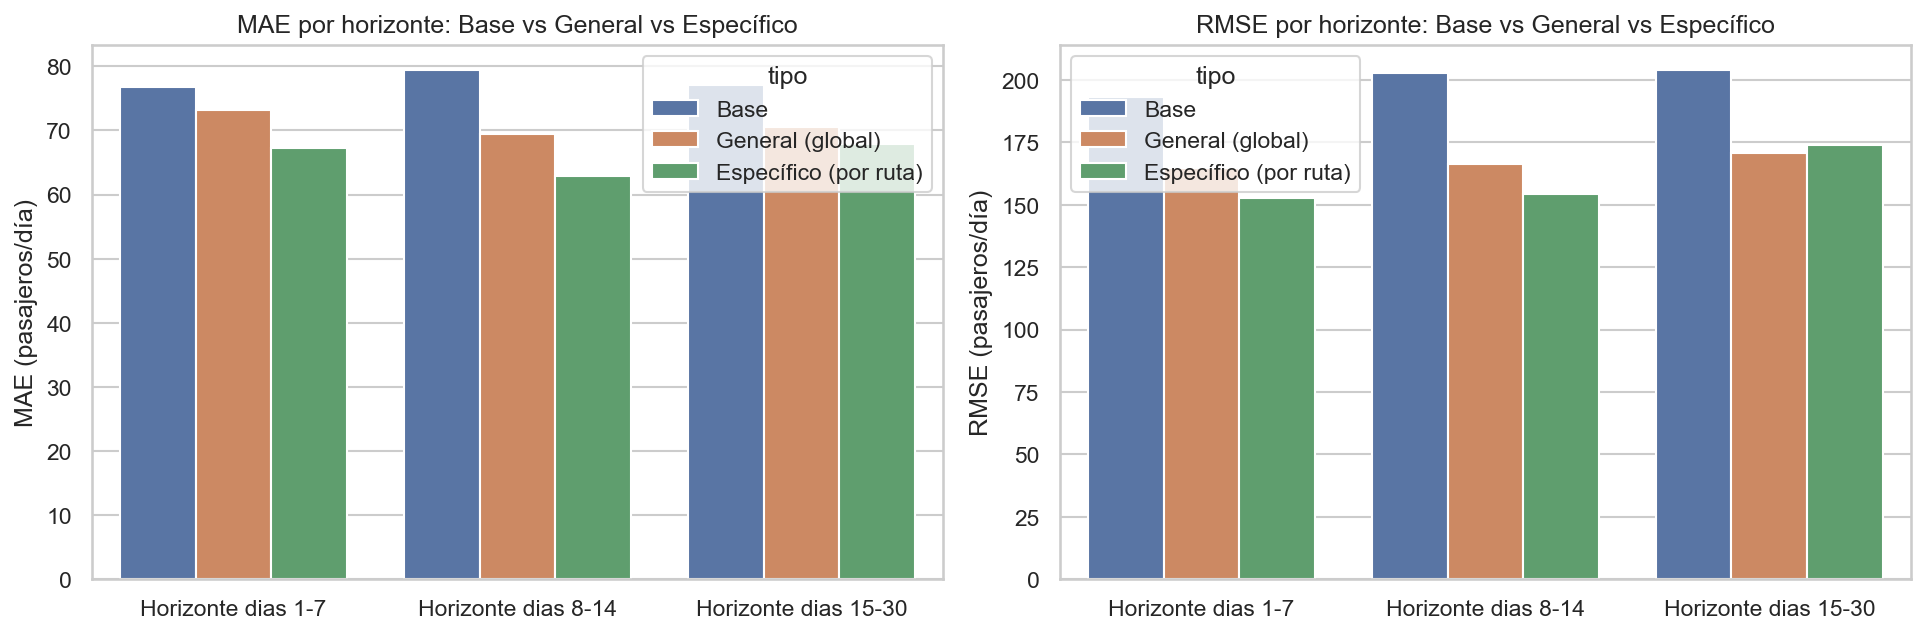
\includegraphics[width=0.90\linewidth]{../figures/ref_01_error_por_horizonte.png}
\caption{Evolución del error (MAE y RMSE) a lo largo del horizonte $h \in \{1, \dots, 30\}$ días comparando los modelos de referencia.}
\label{fig:ref_horizonte}
\end{figure}

\begin{figure}[H]
\centering
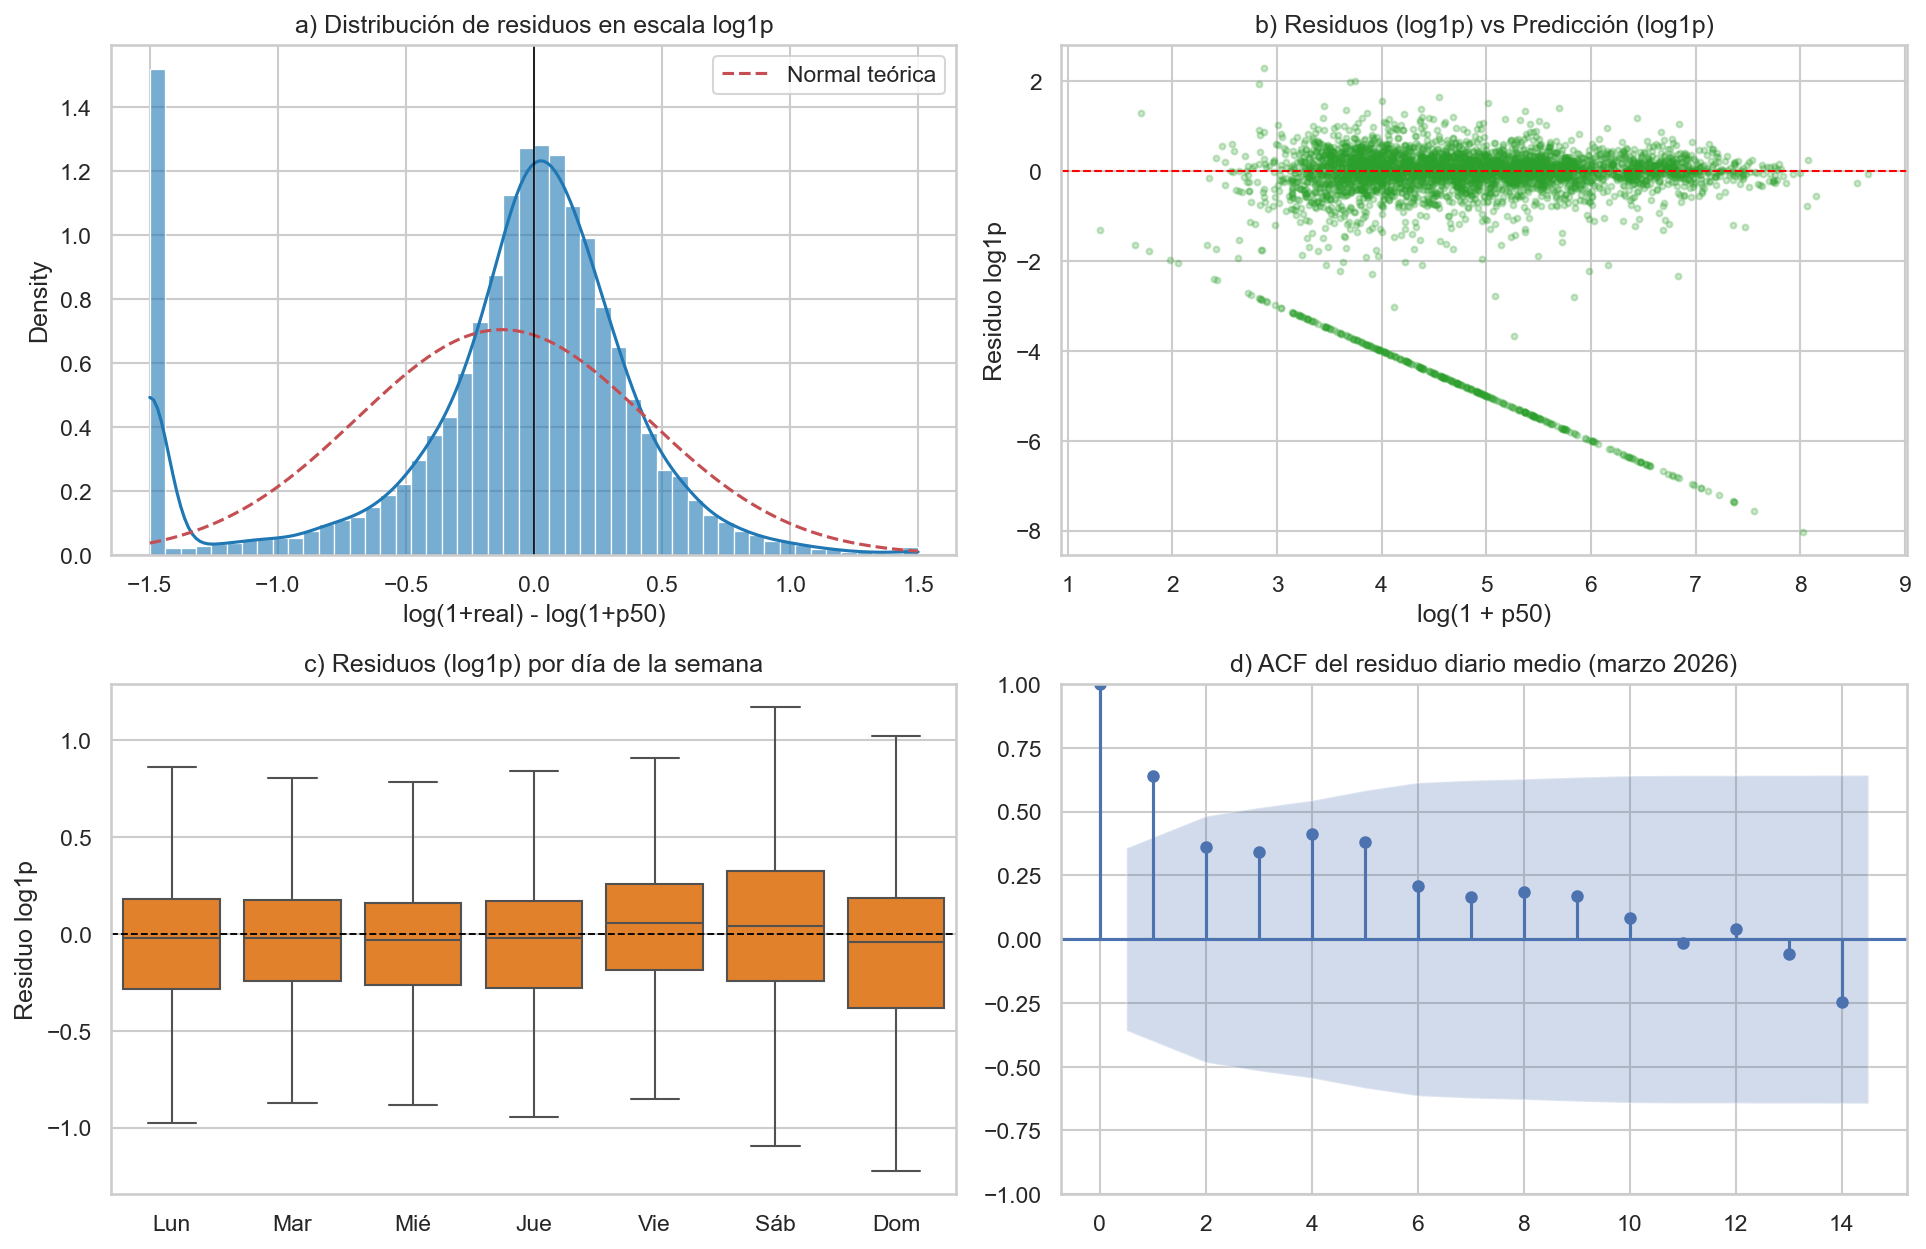
\includegraphics[width=0.90\linewidth]{../figures/ref_02_diagnostico_residuos.png}
\caption{Diagnóstico de residuos del modelo de referencia en validación y prueba.}
\label{fig:ref_residuos}
\end{figure}

\begin{figure}[H]
\centering
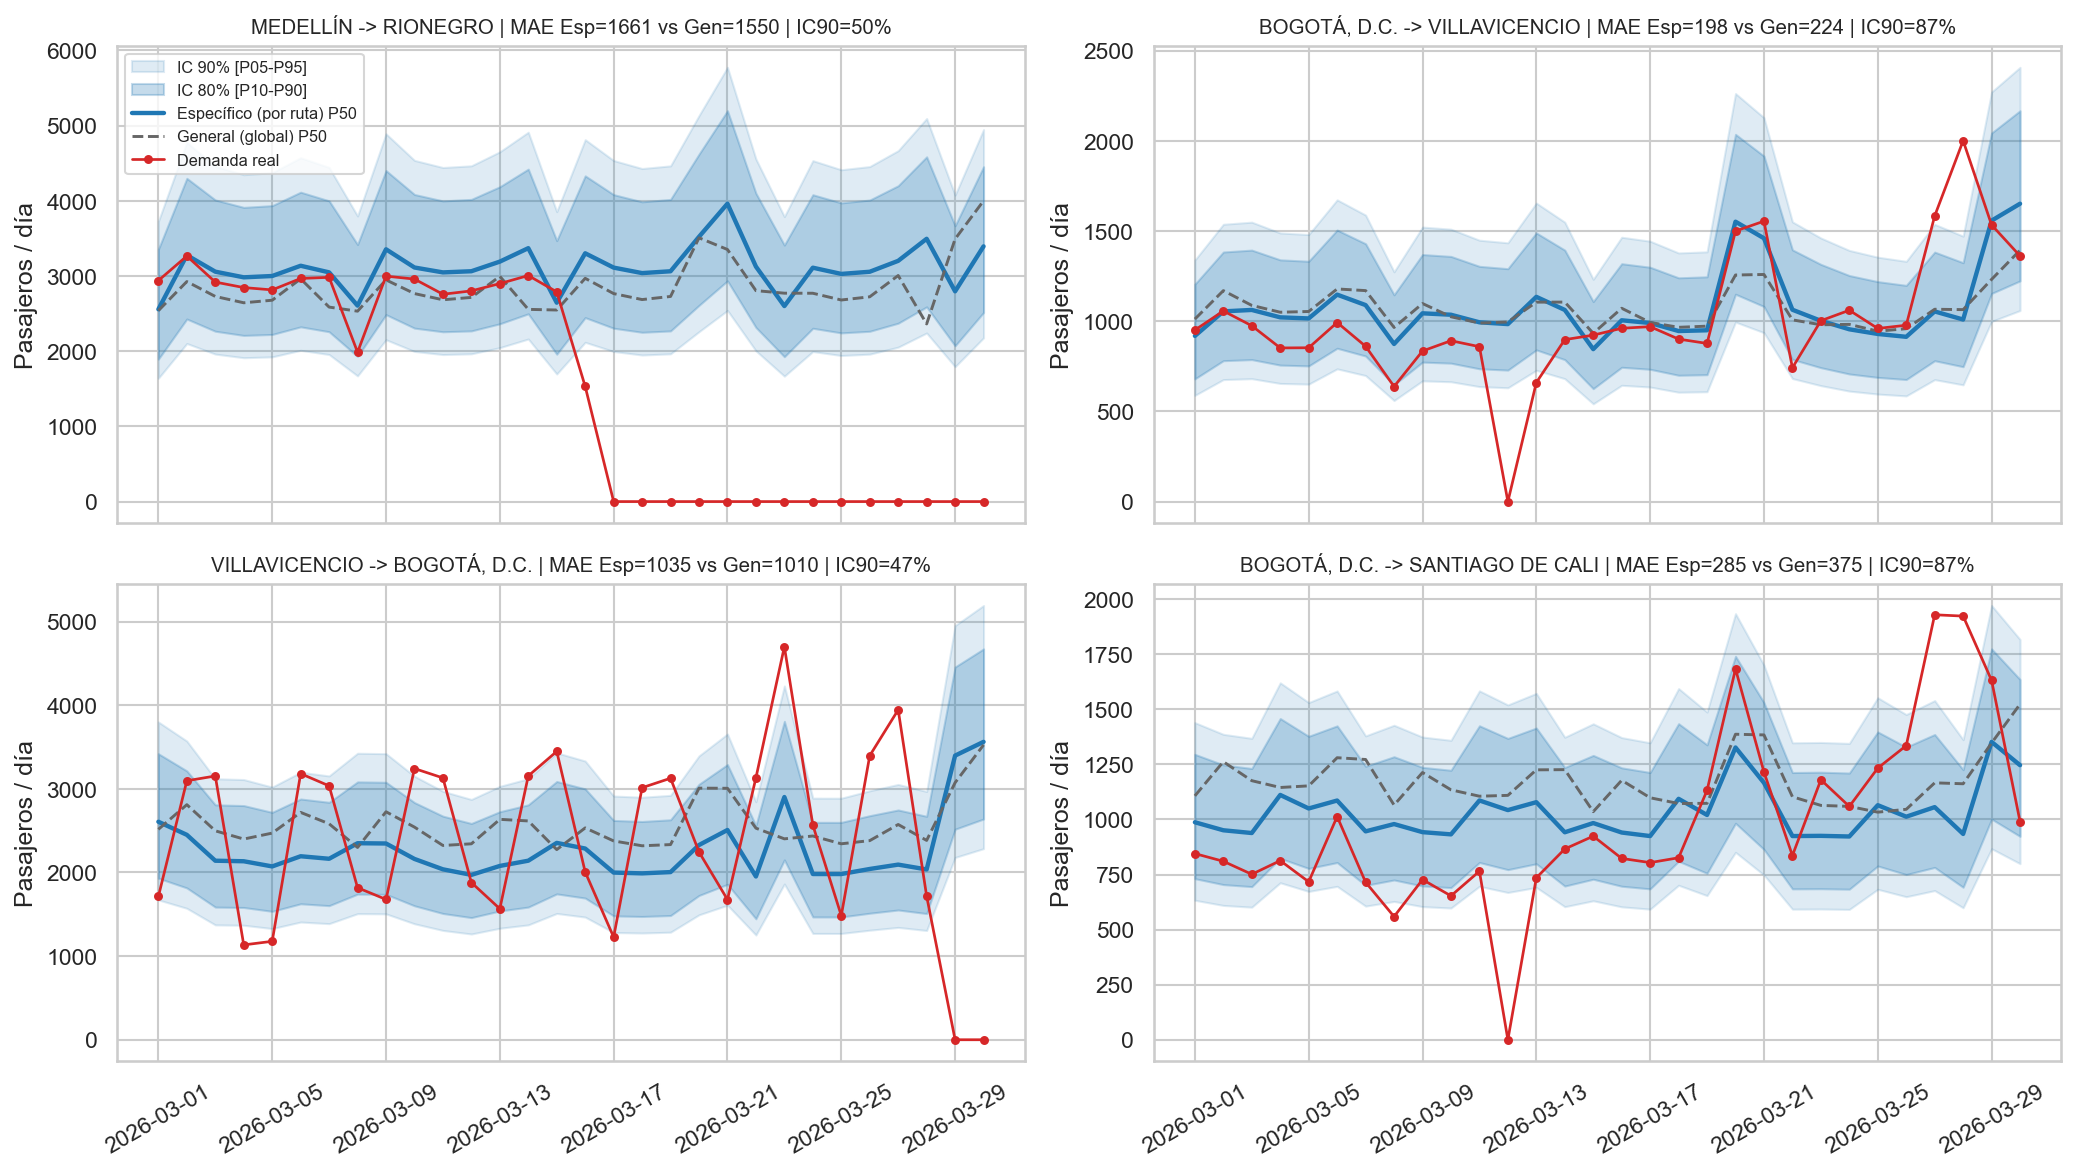
\includegraphics[width=0.92\linewidth]{../figures/ref_03_pronosticos_e_ic_mar2026.png}
\caption{Pronósticos a 30 días (marzo de 2026) con intervalos de incertidumbre ($P_{10}\text{--}P_{90}$ y $P_{05}\text{--}P_{95}$) frente a la demanda real observada.}
\label{fig:ref_mar2026}
\end{figure}

% ==============================================================================
\section{Puente hacia Redes Neuronales: ¿Qué Debe Superar el Modelo Profundo?}
% ==============================================================================

El GLM Poisson Específico por Ruta constituye una línea base exigente ($\text{MAE}=66.55$, $\text{MASE mediano}=0.8836$), pero exhibe cuatro limitaciones estructurales que motivan el uso de \textbf{Redes Neuronales (MLP, LSTM/GRU o CNN-1D)}:

\begin{enumerate}[leftmargin=1.5em]
    \item \textbf{Aislamiento entre rutas vs. \textit{Embeddings}:} el GLM específico entrena 848 modelos aislados que no transfieren conocimiento entre rutas vecinas o similares. Una red neuronal global con capas de \textit{embedding} para \texttt{ruta\_id} puede aprender representaciones latentes compartidas manteniendo especificidad direccional.
    \item \textbf{Interacciones no lineales:} en un GLM, el efecto de un puente festivo es el mismo en temporada baja que en temporada de mitad de año (en escala logarítmica). Una red neuronal puede capturar interacciones no lineales entre calendario, tendencia reciente y nivel de tránsito.
    \item \textbf{Dependencias secuenciales multi-horizonte:} las arquitecturas recurrentes (LSTM/GRU) o convolucionales (CNN-1D) procesan la ventana histórica reciente como una secuencia continua en lugar de rezagos discretos aislados, y pueden emitir directamente el vector completo de 30 días $\hat{\mathbf{y}}_{t_0+1:t_0+30}$.
    \item \textbf{Aprendizaje directo de cuantiles (\textit{Pinball Loss}):} en lugar de calibrar cuantiles \textit{a posteriori} con \textit{offsets} constantes por \textit{tier}, una red neuronal puede entrenarse directamente con la función de pérdida Pinball multi-cuantil ($\{P_{05}, P_{10}, P_{50}, P_{75}, P_{90}, P_{95}\}$), ajustando el ancho de la banda de incertidumbre de forma dinámica según el día y el calendario (ej. bandas más amplias en Semana Santa que en un martes ordinario).
\end{enumerate}

\end{document}
